\section{Analysis}

\subsection{What trends, correlations, and/or patterns do you see in the data?}

Different trends were observed for different data. This section will outline the results of our analysis for the three crops.

\subsubsection{Poultry}

The data frame used for the final analysis contained eight observations.
When the prices and production were plotted using a scatterplot, a clear linear relationship was observed.
The scatterplot and trendline for this relationship can be observed in Figure \ref{fig:chicken_scatter}.
Using the statsmodels package in Python, we determined the coefficients for the linear model using the ordinary least squares (OLS) approach. The output from the regression can be viewed in Figure \ref{fig:chicken_ols}.

The null hypothesis for this test was that no relationship exists between price and production.

The result of this analysis supports the rejection of the null hypothesis, which was there is no effect of prices on production
the model’s intercept was found to be 26.4810 and the coefficient for the prices variable is 50.9459
Production = 26.4810 + 50.9459 x Price
The F-staticic for this model was 12.47 and the changes of observing this statistic under a normal distribution is less than 0.05 %. Therefore, with a p-value set to 0.05, we would reject the null hypothesis.
The R2 is 0.675 which means approximately 67% of the variance of the data can be accounted for by this model.

\subsubsection{Hog}

\subsubsection{Wheat}



\begin{figure}
    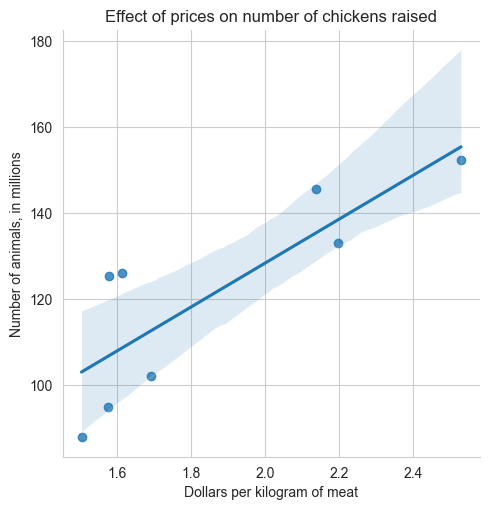
\includegraphics[width=\linewidth]{chicken_scatter}
    \caption{A scatter plot of chicken prices vs. chicken production.}
    \label{fig:chicken_scatter}
\end{figure}



\begin{figure}
    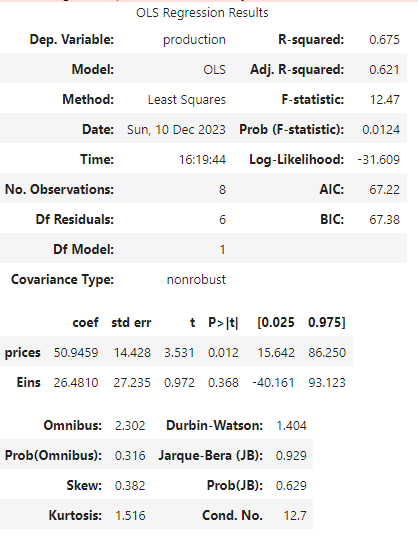
\includegraphics[width=\linewidth]{chicken_ols_results}
    \caption{Results from an Ordinary Least Squares Regression.}
    \label{fig:chicken_ols}
\end{figure}